\chapter{Development Environment}

\section{Prerequisites}
\subsection{Java}
Java SE 6 or later is required. The setup and installation of Java SE 6 is typically
operating system specific, so consult your OS provider. 

\subsection{Ruby}
The Ruby scripting language is required for the source project generation templates. The setup
and installation of Ruby is typically operating system specific, so consult your OS provider.  
Additional ruby plugins (gems) are also required to support the template system (choice,
xml-simple).

\subsection{MySQL}
MySQL is required to support the installation of the Openfire XMPP server.
Download and Installation information is available at :

\begin{center}
http://www.mysql.com
\end{center}

\subsection{Openfire}
The Openfire XMPP server is required to support the construction of virtual
networks within the TINOS platform. Download and Installation information
is available at :

\begin{center}
http://www.igniterealtime.org/projects/openfire
\end{center}

\subsection{WireShark}
WireShark is a tool that is used to examine TINOS network trace logs.
Download and installation information is available at :

\begin{center}
http://www.wireshark.org
\end{center}

\section{Post Installation Steps}
\subsection{Set environment variables}
\subsubsection{JAVA\_HOME}
TINOS uses the JAVA\_HOME environment variable to locate the java executable.
Configure this environment variable to point to the home directory of the Java 5 or 6
installation on your computer.


\section{Directory Layout}

\begin{figure}
\dirtree{%
 .1 USER\_HOME.
 .2 env.sh\DTcomment{User Environment Setup}.
 .2 development\DTcomment{DEV\_HOME - Development Toolchain}.
 .3 build-tools.
 .4 apache-ant-1.7.1\DTcomment{Apache Ant}.
 .4 findbugs-1.3.9\DTcomment{findbugs}.
 .3 springsource\DTcomment{SpringSource Tools}.
 .4 virgo-web-server-2.1.0.M01\DTcomment{SERVER\_HOME - Virgo WebServer Directory}.
 .4 sts-2.3.2.RELEASE\DTcomment{Springsource Tool Suite (eclipse)}.
 .2 tinos\DTcomment{TINOS\_HOME - tinos git repository}.
 .3 documentation\DTcomment{Documentation}.
 .3 projects\DTcomment{Project Bundles}.
 .3 repository\DTcomment{Artifact Repository}.
 .3 build\DTcomment{Build Template Scripts}.
}
\caption{High Level Installation Layout}
\end{figure}

\section{Environment Settings}
Generally we attempt to isolate environments from each other as a matter of course.
This supports the idea of multiple environments being available for a user dependent
upon what they want to do.

To support this idea, all the enviroment settings for TINOS development are
written into the file env.sh in the development directory. This file can be sourced within
the shell of the user to append the relevant settings to their default shell.

In doing so, the user tailors this shell for the TINOS development environment
and platform. Listings of the relevant settings under the various headings of the
installation are provided just to help join the dots for the reader. A complete env.sh
file is also listed at the end of the document.

\subsection{SERVER\_HOME}
As a convenience it is recommended that you create an environment variable that points
to the Virgo Web Server installation directory. Note that the Virgo Web Server does not
required that such an environment variable has been set. This variable may have any
name of your choosing.The following documentation assumes that the variable is
named SERVER\_HOME.

\subsection{DEV\_HOME}
As a convenience it is recommended that you create an environment variable that points
to the directory that contains the development environment tooling. This variable may
have any name of your choosing.The following documentation assumes that the variable
is named DEV\_HOME.

The location of the DEV\_HOME directory is typically "development" located in the user
home directory. However, it is up to the user to choose this location.

\subsection{TINOS\_HOME}
As a convenience it is recommended that you create an environment variable that points
to the directory that contains the tinos git repository. The following documentation assumes
that the variable is named TINOS\_HOME.

The location of the TINOS\_HOME directory is typically "tinos" located in the user home
directory. It is up to the user to choose this location.

\section{Directory Setup}
\begin{description}
 \item[Task] Setup the development toolchain.
 \item[\$] mkdir development; cd development
 \item[\$] export DEV\_HOME=`pwd`
 \item[\$] mkdir build-tools
 \item[\$] mkdir springsource
 \item[\$] echo \$DEV\_HOME
 \item[Note] Copy down the value of DEV\_HOME as it will need to be added to the
 env.sh file.
\end{description}

\begin{description}
 \item[Task] Pull down the TINOS repository from GitHub
 \item[\$] cd
 \item[\$] git clone \$ GitHub Repository URL for TINOS \$
 \item[\$] cd tinos
 \item[\$] export TINOS\_HOME=`pwd`
 \item[\$] echo \$TINOS\_HOME
 \item[Note] Copy down the value of TINOS\_HOME as it will need to be added to the
 env.sh file.
\end{description}

\section{Install Virgo WebServer}

The current version of Virgo is virgo-web-server-2.1.0.M01.

TINOS is loaded and executed within the Virgo WebServer platform. It is
recommended that the Virgo WebServer is installed in the DEV\_HOME
directory as TINOS users will need to interact with this server directly in order
to load and execute TINOS nodes. Download and installation information
is available at :

\begin{center}
http://www.eclipse.org/virgo
\end{center}

\subsection{Installation}
\begin{description}
 \item[Task] Download the Virgo Web Server from Eclipse.
 \item[URL] http://www.eclipse.org/virgo/download
 \item[Note] Assuming the zip file is downloaded to the HOME directory.
 \item[\$] cd \$DEV\_HOME/springsource
 \item[\$] unzip \$HOME/virgo-web-server-2.1.M01.zip
 \item[Note] This will extract the virgo server into virgo-web-server-2.1.0.M01 directory.
 \item[\$] cd virgo-web-server-2.1.0.M01/bin
 \item[Note] Create a file called setenv.sh and place the following in it.
\begin{verbatim}
# Workaround (OSX)
# Java JVM issue in relation to the churn of the PERM cache.
export JAVA_OPTS="-Xms64m -Xmx512m -XX:PermSize=128m -XX:MaxPermSize=756m"
\end{verbatim}
\end{description}

\subsection{Environment Settings}
\begin{verbatim}
# Virgo Settings
export SERVER_HOME=$DEV_HOME/springsource/virgo-web-server-2.1.0.M01
export SERVER_EXEC=$SERVER_HOME/bin
\end{verbatim}

\section{Ant}
The current version of Ant is apache-ant-1.7.1.
\subsection{Installation}
\begin{description}
 \item[Task] Download the Apache Ant from Apache.Org.
 \item[URL] http://ant.apache.org/bindownload.cgi
  \item[Note] Assuming the zip file is downloaded to the HOME directory.
 \item[\$] cd \$DEV\_HOME/build-tools
 \item[\$] unzip \$HOME/apache-ant-1.7.1-bin.zip
 \item[Note] This will extract the ant into the directory: apache-ant-1.7.1
\end{description}

\subsection{Environment Settings}
\begin{verbatim}
# Ant Settings
export ANT_HOME=$DEV_HOME/build-tools/apache-ant-1.7.1
# Workaround (OSX)
# Java JVM issue in relation to the churn of the PERM cache.
export ANT_OPTS="-Xms64m -Xmx512m -XX:PermSize=128m -XX:MaxPermSize=756m"
export ANT_EXEC=$ANT_HOME/bin
\end{verbatim}


\section{Findbugs}
The current version of Findbugs is findbugs-1.3.9.
\subsection{Installation}
\begin{description}
 \item[Task] Download the findbugs from 
 \item[URL] http://findbugs.sourceforge.net/downloads.html
 \item[Note] Assuming the zip file is downloaded to the HOME directory.
 \item[\$] cd \$DEV\_HOME/build-tools
 \item[\$] tar xzvf \$HOME/findbugs-1.3.9.tgz
 \item[Note] This will extract the findbugs into the directory: findbugs-1.3.9
\end{description}

\subsection{Environment Settings}
\begin{verbatim}
export FINDBUGS_HOME=$DEV_HOME/build-tools/findbugs-1.3.9
export FINDBUGS_EXEC=$FINDBUGS_HOME/bin
\end{verbatim}

\section{SpringSource Tool Suite}
Install the Spring Tool Suite (SpringSource branded version of \textit{Eclipse}),
 it is invoked on the command line as ''STS``.

\textbf{Note: } The GUI toolchain (STS/Eclipse) will be updated shortly to handle
the upgrade changes from Spring dm to Virgo. Command line operation is not affected,
it is only the integration with GUI development tools. So expect changes here. 

\begin{description}
\item[Task] Download SpringSource Tool Suite.
\item[URL] http://www.springsource.com/products/springsource-tool-suite-download
\item [\$] cd \$DEV\_HOME/springsource
\item [\$] unzip \$HOME/sts-2.3.2.RELEASE.zip
\item [Note] This will extract into the following directory : sts-2.3.2.RELEASE
\end{description}

\subsection{Environment Settings}
\begin{verbatim}
export STS_HOME=$DEV_HOME/springsource/sts-2.3.2.RELEASE
\end{verbatim}



\section{Overall Environment Settings}
All of the environmental settings from above combined and integrated. Typically
this file is imported into the users shell whenever they wish to use the environment.

\begin{description}
 \item[Task] Append the TINOS Environment settings, a sample env.sh file is shown
 below.
 \item[\$] cd
 \item[\$] . ./env.sh
 \item[Joy] Ready to rock and roll!.
\end{description}


\begin{verbatim}
# Development Toolchain Location
export DEV_HOME=$HOME/development

# TINOS Git Repository
export TINOS_HOME=$HOME/github/tinos

# Java JDK/JRE (OSX)
export JAVA_HOME=/Library/Java/Home

# Virgo 
export SERVER_HOME=$DEV_HOME/springsource/virgo-web-server-2.1.0.M01
export SERVER_EXEC=$SERVER_HOME/bin

# STS
export STS_HOME=$DEV_HOME/springsource/sts-2.3.2.RELEASE

# Ruby Settings
export RUBYOPT=rubygems

# Ant Settings
export ANT_HOME=$DEV_HOME/build-tools/apache-ant-1.7.1
# Workaround (OSX)
# Java JVM issue in relation to the churn of the PERM cache.
export ANT_OPTS="-Xms64m -Xmx512m -XX:PermSize=128m -XX:MaxPermSize=756m"
export ANT_EXEC=$ANT_HOME/bin

# Findbugs
export FINDBUGS_HOME=$DEV_HOME/build-tools/findbugs-1.3.9
export FINDBUGS_EXEC=$FINDBUGS_HOME/bin

# Setup Path
export PATH=$JAVA_HOME/bin:$ANT_EXEC:$SERVER_EXEC:$PATH
export PATH=$STS_HOME:$FINDBUGS_HOME:$PATH

# Alias
export EDITOR=vim
alias vi='vim'
\end{verbatim}

\section{Openfire Database Installation}
Before the installation of Openfire, a database user and database for the
Openfire server must be created.

\begin{description}
\item[Task] Create database user and database
\item [Note] Create a database
\item [\$] mysql -u root -p
\item [mysql\$] create database openfire character set utf8;
\item [Note] Create a user
\item [mysql\$] grant all on openfire.* to openfire@localhost identified by 'openfire';
\item [mysql\$] commit; exit;
\end{description}

\section{OpenFire 3.6.4}
Install the OpenFire server as instructed on their website. Once this is completed,
start the server and then follow the instructions below to configure the server.


\section{OpenFire Configuration}
In order to complete the configuration of the OpenFire server, a web browser must be
used to step through the server setup screens.

\begin{description}
 \item [Task] Configure the OpenFire server with a web browser.
 \item [Browser] Enter the following URL to start the configuration.
 \item [URL] http://localhost:9090
\end{description}

\begin{description}
\item [Browser] Select the English language and click Continue.
\end{description}
\begin{center}
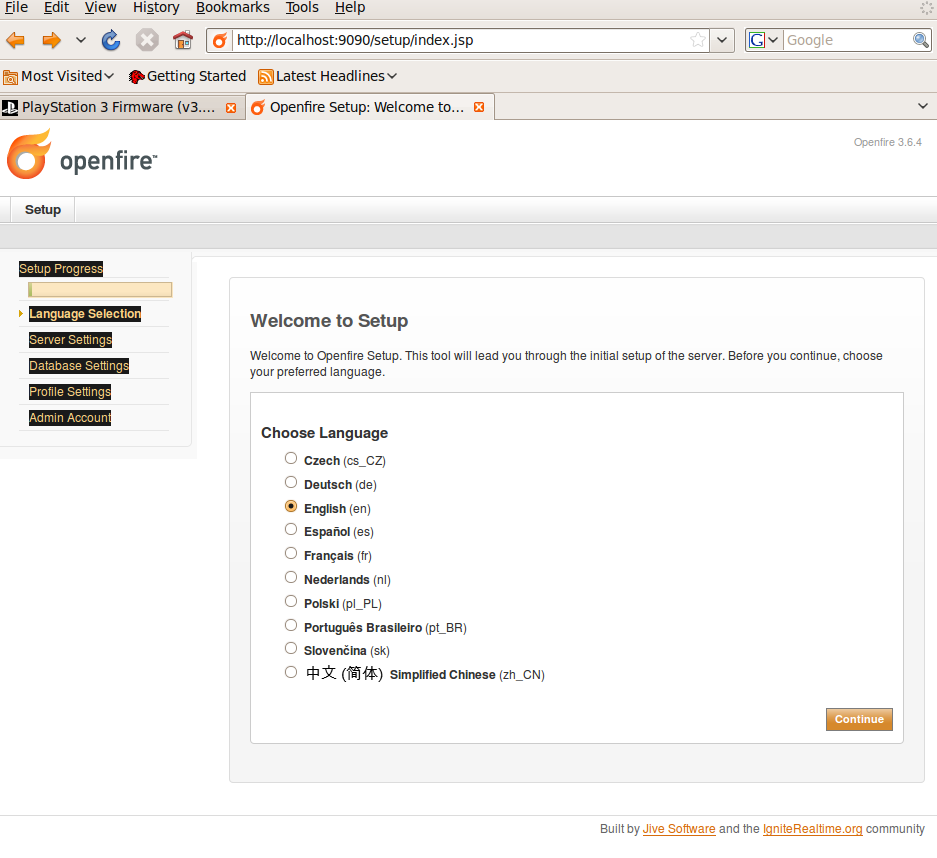
\includegraphics[scale=0.5]{figs/deploy/openfire-1.png} 
\end{center}

\begin{description}
\item [Task] Configure the Server Settings
\item [Browser] Enter ''localhost`` as the domain and leave the other settings unchanged.
\item [Browser] Click Continue
\end{description}
\begin{center}
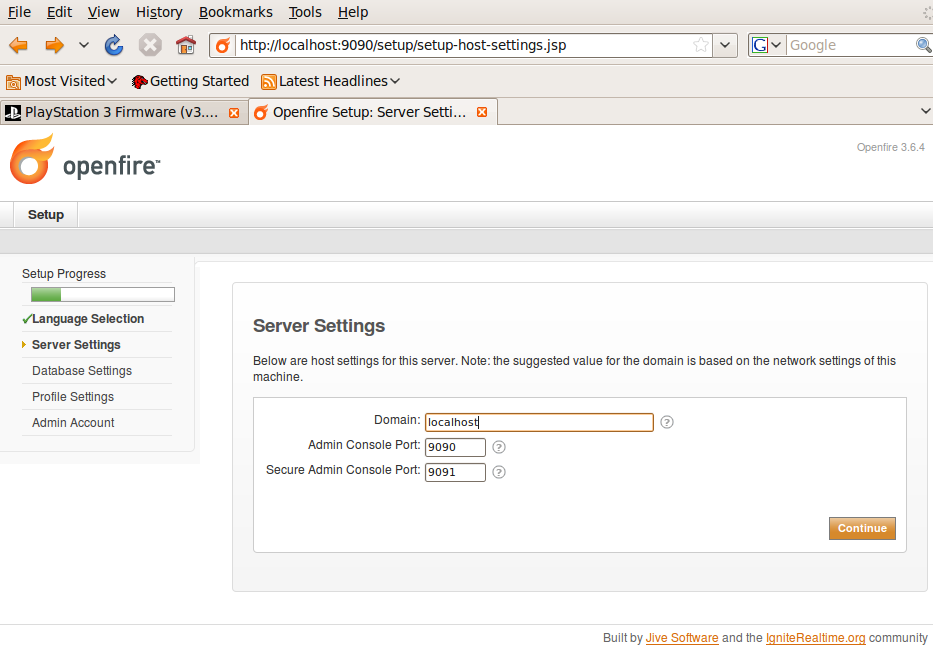
\includegraphics[scale=0.5]{figs/deploy/openfire-2.png} 
\end{center}


\begin{description}
\item [Task] Configure the Database Settings
\item [Browser] Select ''Standard Database Connection``
\item [Browser] Click Continue
\end{description}
\begin{center}
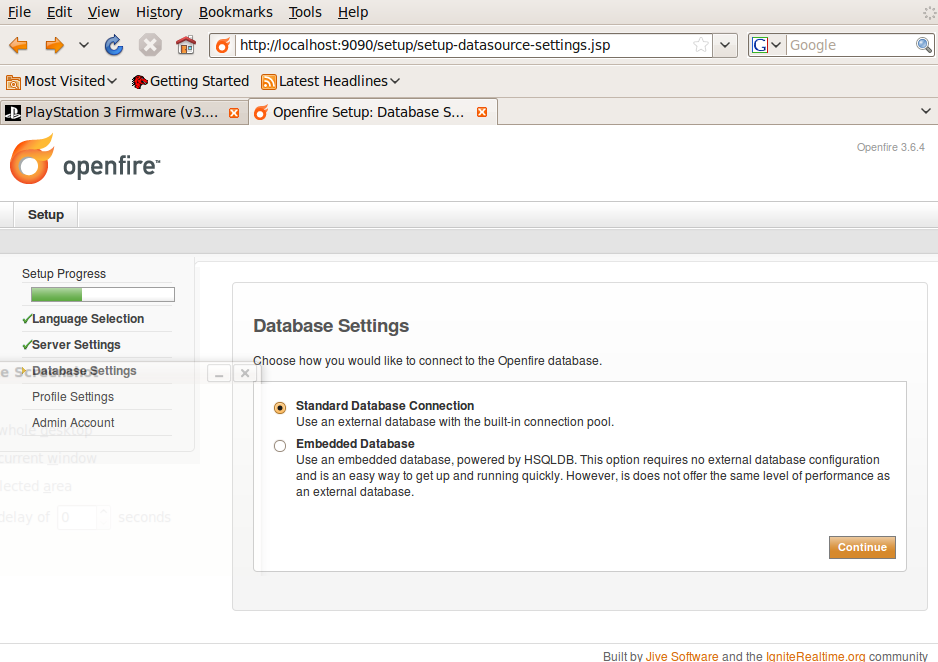
\includegraphics[scale=0.5]{figs/deploy/openfire-3.png} 
\end{center}

\begin{description}
\item [Task] Configure the Standard Database Settings
\item [Browser] Select ''MySQL`` in the Database Driver presets.
\item [Browser] Edit the Database URL to ''jdbc:mysql://localhost:3306/openfire``
\item [Browser] Edit the Username to ''openfire``
\item [Browser] Edit the Password to ''openfire``
\item [Browser] Click Continue
\item[Note] The database settings reflect those configured earlier.
\end{description}
\begin{center}
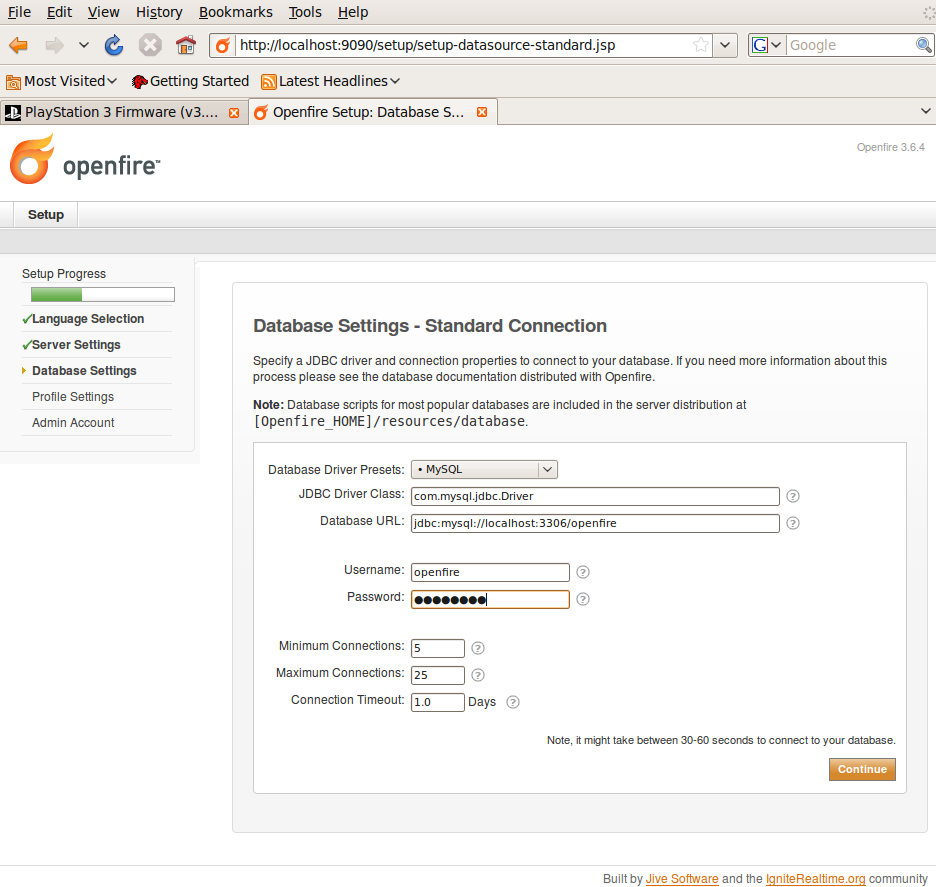
\includegraphics[scale=0.5]{figs/deploy/openfire-4.png} 
\end{center}


\begin{description}
\item [Task] Configure the Profile Settings
\item [Browser] Select ''Default``
\item [Browser] Click Continue
\end{description}
\begin{center}
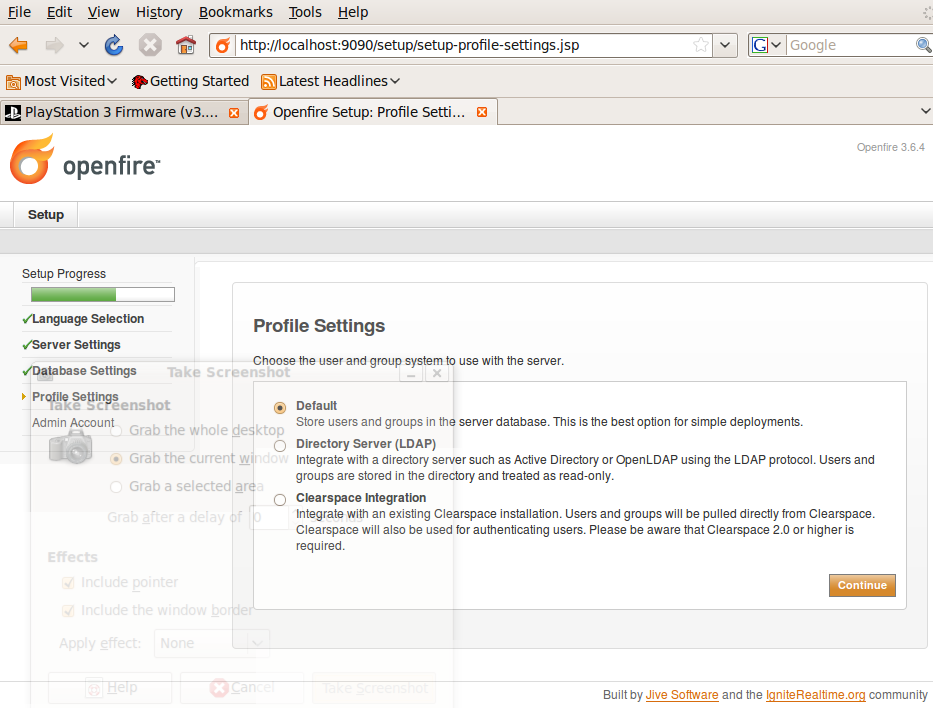
\includegraphics[scale=0.5]{figs/deploy/openfire-5.png} 
\end{center}

\begin{description}
\item [Task] Configure the Administrator Settings
\item [Browser] Click ''Skip this step``
\item [Note] This is only to complete the installation configuration. In the next steps
a database import with change this value to the default.
\end{description}
\begin{center}
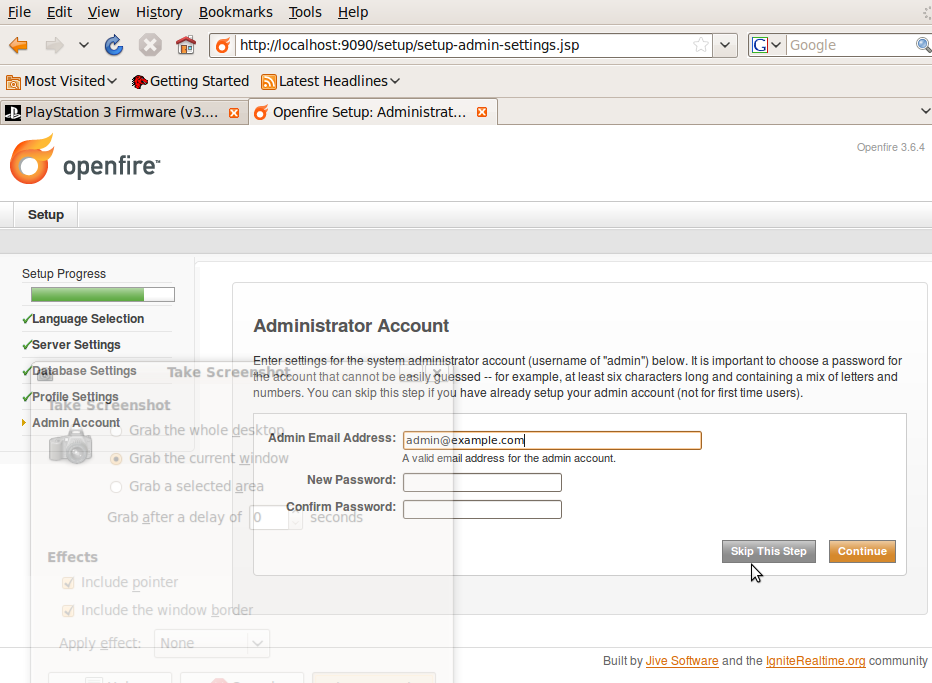
\includegraphics[scale=0.5]{figs/deploy/openfire-6.png} 
\end{center}

\begin{description}
\item [Task] Setup Complete
\item [Browser] Setup should now be complete.
\end{description}
\begin{center}
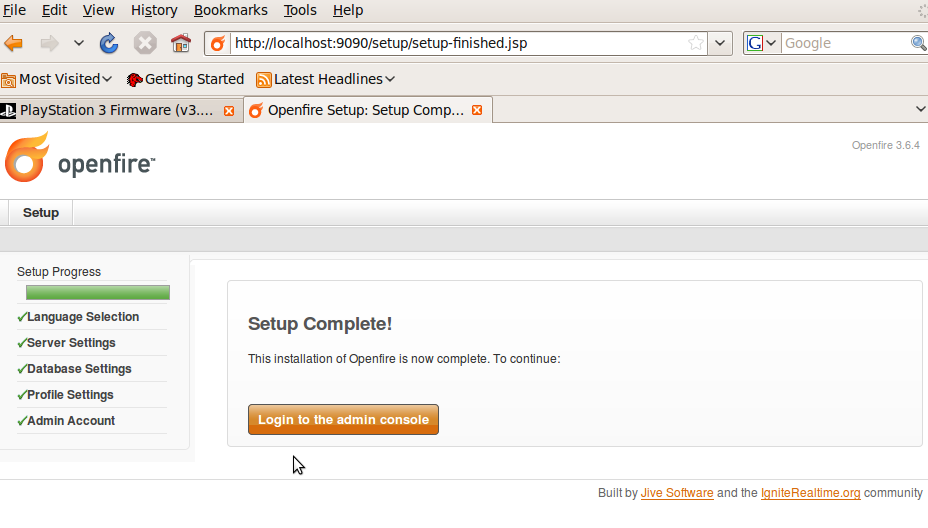
\includegraphics[scale=0.5]{figs/deploy/openfire-7.png} 
\end{center}

\section{OpenFire Demo Configuration}
The OpenFire server must be configured to match the requirements of the
pre-canned demo applications. As such the existing database will be cleared and a
valid configuration loaded in its place. This saves the long and tedious configurations
required within OpenFire for all the users, groups and chatrooms.

\begin{description}
\item [Task] Shutdown the OpenFire Server
\item [Note] Check the Openfire documentation to shutdown the server for your OS.
\item [Task] Clear the old database.
\item [\$] mysql -u root -p
\item [mysql\$] drop database openfire;
\item [mysql\$] create database openfire character set utf8;
\item [mysql\$] commit; exit;
\item [Task] Load the new database
\item [\$] mysql -u openfire -p openfire $<$
 \$TINOS\_HOME/documentation/demo/simple-ping/db/openfire.db
\item[Note] You will be prompted for the password : ''openfire``
\item [Task] Start the OpenFire Server
\item [Note] Check the Openfire documentation to start the server for your OS.
\item [Task] Login to the OpenFire Administration Console
\item [Browser] Goto URL: http://localhost:9090
\item [Browser] Username : ''admin``, Password : ''12345``
\item [Note] You can change the password afterwards if you wish.
\end{description}
\begin{center}
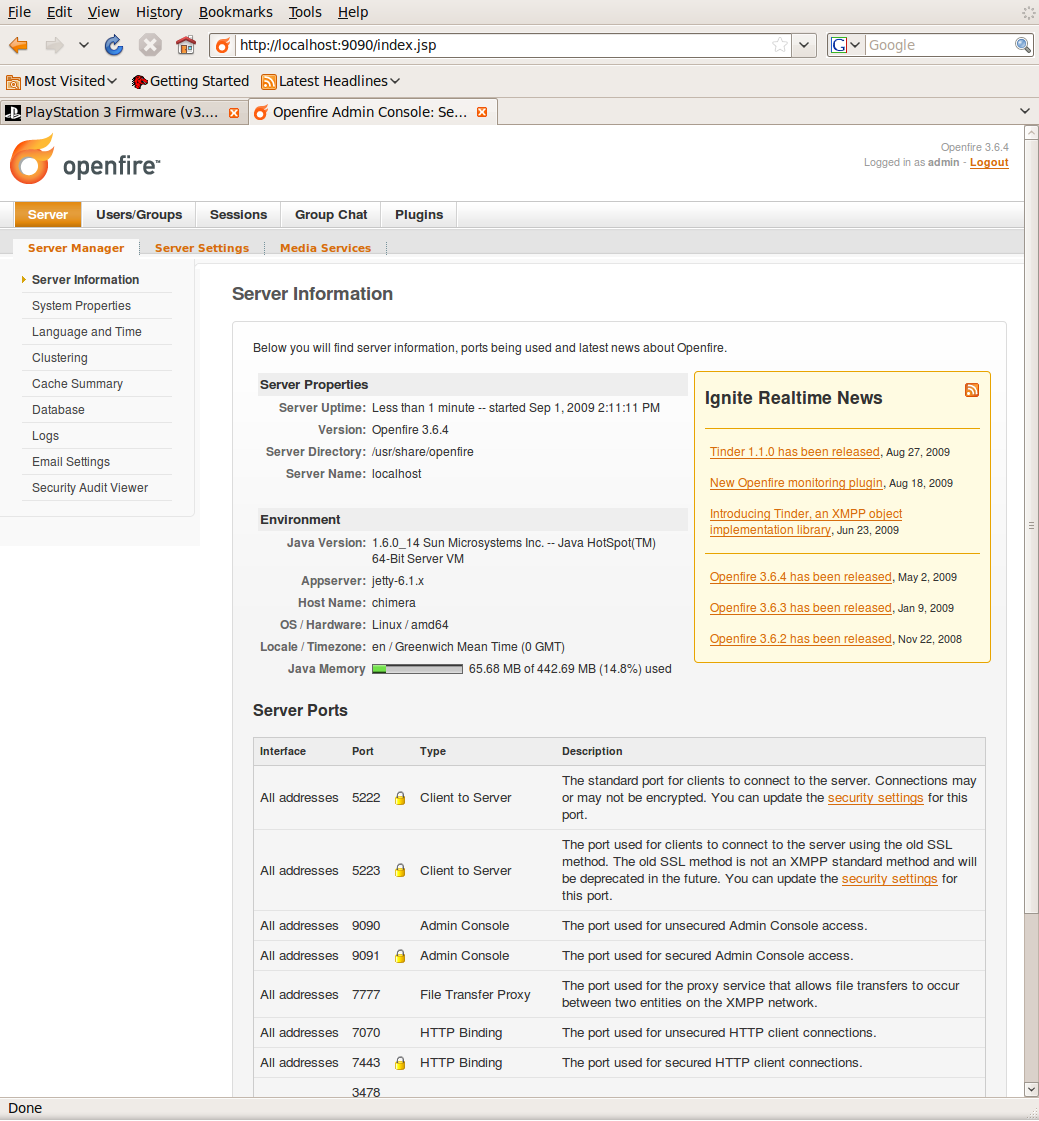
\includegraphics[scale=0.4]{figs/deploy/openfire-8.png} 
\end{center}

\section{Virgo Server Configuration}

\begin{description}
\item [Task] Configure logging/trace for the Jnode applications
\item [\$] . \$HOME/env.sh
\item [\$] cd \$SERVER\_HOME
\item [\$] vi config/serviceability.xml
\item [Note] Add the following lines between the TINOS Start / End to the end
of the serviceability.xml file. To exit ''vi'' use the key sequence [ESC]:wq[RETURN]
\begin{verbatim}
<!-- TINOS - Start -->
        <logger level="DEBUG" additivity="false" name="org.jnode">
                <appender-ref ref="SIFTED_LOG_FILE" />
        </logger>
        <logger level="DEBUG" additivity="false" name="org.pouzinsociety">
                <appender-ref ref="SIFTED_LOG_FILE" />
        </logger>
<!-- TINOS - End -->

        <root level="WARN">
                <appender-ref ref="SIFTED_LOG_FILE" />
\end{verbatim}
\item [Task] Add the demo bundles
\item [\$] cp \$TINOS\_HOME/documentation/demo/simple-ping/bundles/* repository/usr
\item [Task] Add the Plan files
\item [\$] cp \$TINOS\_HOME/documentation/demo/simple-ping/plans/* .
\end{description}

\section{XMPP/Jabber IM Client}
Once configured you can use the IM Client to visually see the presence of the nodes
within the demo networks, as well as sit in the networks (via chatrooms) and see the
interactions. Super cheap and cheerful GUI.

The following clients have been tested successfully (Ubuntu : Pidgin, OSX : iChat,
 Windows : Spark). However as long as your client supports XMPP/Jabber, it should be
fine.

\begin{description}
\item [Task] Configure Your IM Client (XMPP/Jabber Capable)
\item[Account Details]
\item[Server] Protocol: XMPP, Domain: localhost, Server: localhost
\item[Buddy] User: human, Password: Human
\item[Note] Below are sample configuration screens from the Pidgin client.
\end{description}
\begin{center}
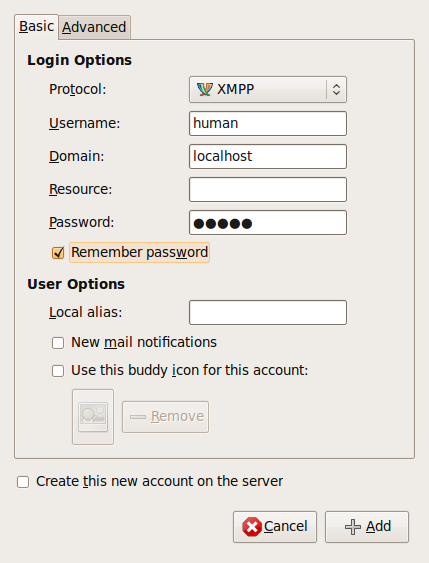
\includegraphics[scale=0.5]{figs/deploy/pidgin-1.png} 
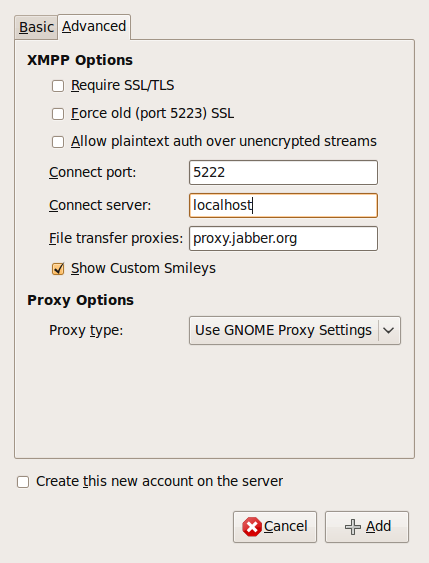
\includegraphics[scale=0.5]{figs/deploy/pidgin-2.png} 
\end{center}

\begin{description}
\item [Task] Ensure you can see Offline Buddies
\item[Note] Sample Buddy Roster from Pidgin Client.
\end{description}
\begin{center}
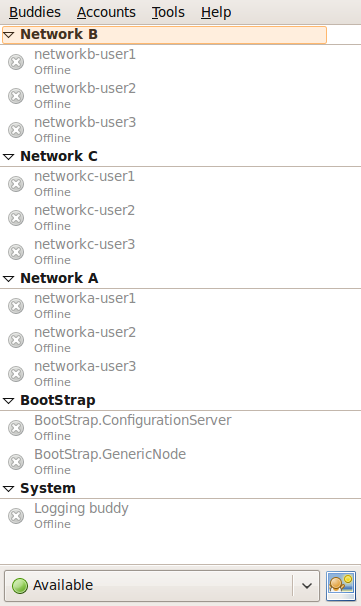
\includegraphics[scale=0.5]{figs/deploy/pidgin-3.png} 
\end{center}

\section{TINOS - Simple Ping Demo}

For the first initial loading of the demo - the following actions must be performed
in exact sequence. This is primarily to make life easier for the person giving /
viewing the demo as everything will start in an order that will match a presentation.

\begin{description}
\item [Task] Start the Virgo Server
\item[\$] . \$HOME/env.sh
\item[\$] cd \$SERVER\_HOME/bin
\item[\$] ./startup.sh --clean
\item[Note] Wait for this to complete.
\end{description}


\textit{If you are doing a demo - it is most useful to have the IM Client open
during the demo as you will be able to watch the bootstrap in progress (via presence)
and also the nodes as they are configured and come online.
}

\textit{ The demo scenario is the almost the most basic possible with a simple
ping scenario being enacted between the nodes but in order to do this the nodes,
drivers, stacks (IPv4/TCP/Socket API/Name Resolver/Routes) and simple traffic
generator (ping) are configured and enabled within the OSGi environment.
}

\textbf{This is a starting point for more elaborate scenarios but more importantly
it provides a simple demo that validates environment setup is correct.}

\subsection{Initial Run of the Demo}
\begin{description}
\item [Task] Start Your IM Client \& login as human
\item [Task] New Terminal Shell - Load the Demo Applications
\item[\$] . \$HOME/env.sh
\item[\$] cd \$SERVER\_HOME
\item[Task] Start the BootStrap configuration Manager
\item[\$] mv org.pouzinsociety.config.manager.plan pickup
\item[Note] Watching the other terminal - wait until the application in successfully loaded.
\item[Task] Start the Logger Agent
\item[\$] mv org.pouzinsociety.logger.plan pickup
\item[Note] Watching the other terminal - wait until the application in successfully loaded.
\item[Task] Start Jnode0
\item[\$] mv org.pouzinsociety.node.plan pickup
\item[Note] Watching the other terminal - wait until the application in successfully loaded.
\item[Note] Wait for IM Buddy - networkb-user1 to come online (Jnode0 fully configured).
\item[Task] Start Jnode1
\item[\$] mv org.pouzinsociety.node1.plan pickup
\item[Note] Watching the other terminal - wait until the application in successfully loaded.
\item[Note] Wait for IM Buddy - networkb-user2 to come online (Jnode1 fully configured).
\item[Note] The logger application will produce PCAP files in the ''/tmp`` directory.
\item[Task] Start WireShark
\item[Note] The file to load into WireShark is ''/tmp/networka@conference.localhost.pcap``
as this will have the ARP/Ping traffic present in it.
\end{description}

\begin{center}
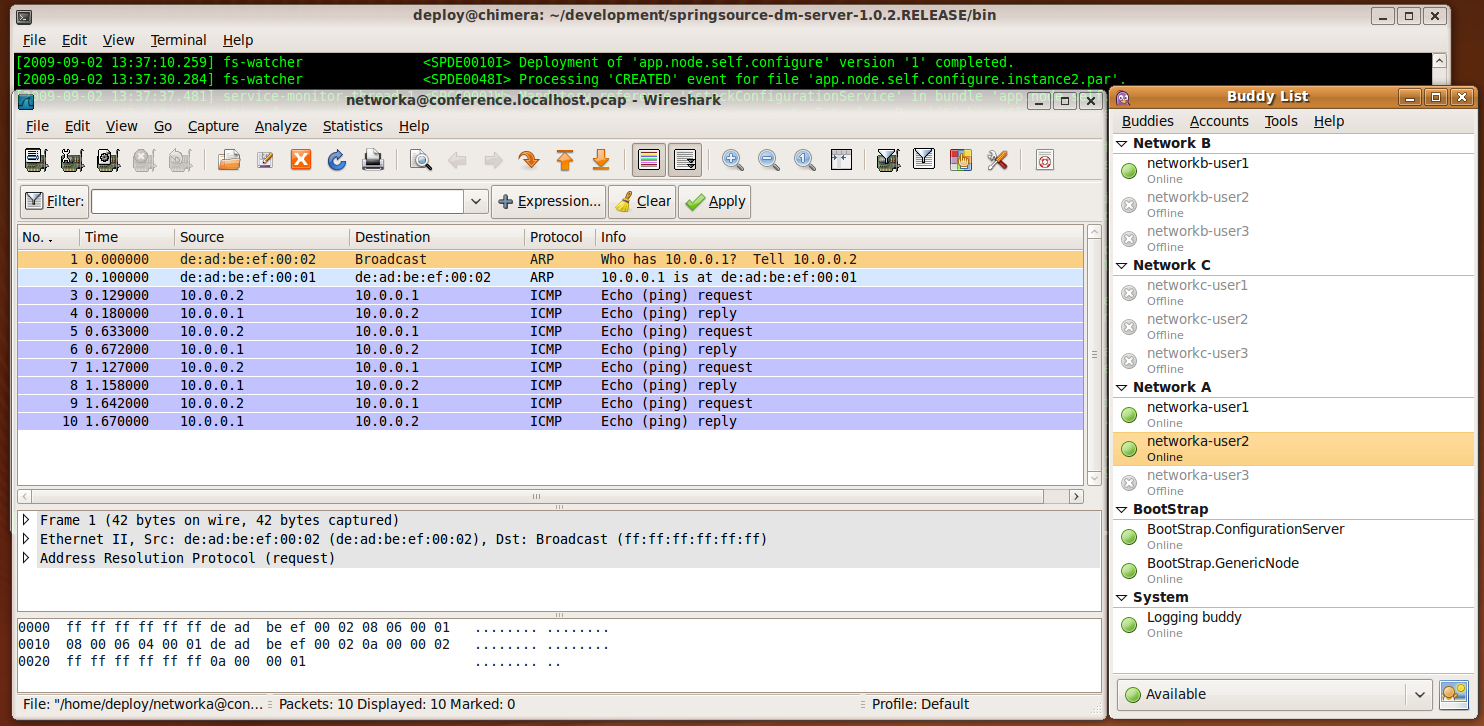
\includegraphics[scale=0.3]{figs/deploy/pidgin-4.png} 
\end{center}

\subsection{Stopping the Virgo Server}
\begin{description}
\item [Task] Stop the Virgo Server
\item [Note] Simply CTRL-C in the shell you started the server.
\end{description}

\subsection{Post-Initial Demo}
\begin{description}
\item [Task] Running it Again
\item [Note] Simply start the server. Do not copy demo plan files into the pickup directory.
The server will automatically pick them up on all the subsequent server startups.
\item[Note] Delete the pcap files under the ''/tmp`` directory.
\end{description}

\section{Useful Links}
\begin{description}
\item[Note] Free Book - OSGi in Practise
\item[URL] http://neilbartlett.name/blog/osgibook/
\item[--] 
\item[Note] SpringSource Enterprise Bundle Repository
\item[URL] http://www.springsource.com/repository/app/
\item[--]
\item[Note] SpringSource dm Server Programmer Guide
\item[URL] http://static.springsource.com/projects/dm-server/1.0.x/programmer-guide/htmlsingle/programmer-guide.html
\item[--]
\item[Note] OSGi Service Platform R4 Specification
\item[URL] http://www.osgi.org/Download/Release4V41?info=nothanks
\item[--]
\item[Note] Tutorial for Spring Dynamic Modules (DM) for OSGi Service Platforms
\item[URL] http://springosgi.googlepages.com/
\end{description}
